%%%%%%%%%%%%%%%%%%%%%%%%%%%%%%%%%%%%%%%%%%%%%%%%%%%%%%%%%%%%%%%%
%%%%%%%%%%%%%%%%%%%%%%%%%%%%%%%%%%%%%%%%%%%%%%%%%%%%%%%%%%%%%%%%
%%%%
%%%% This text file is part of the source of 
%%%% `Introduction to High-Performance Scientific Computing'
%%%% by Victor Eijkhout, copyright 2012
%%%%
%%%% This book is distributed under a Creative Commons Attribution 3.0
%%%% Unported (CC BY 3.0) license and made possible by funding from
%%%% The Saylor Foundation \url{http://www.saylor.org}.
%%%%
%%%%
%%%%%%%%%%%%%%%%%%%%%%%%%%%%%%%%%%%%%%%%%%%%%%%%%%%%%%%%%%%%%%%%
%%%%%%%%%%%%%%%%%%%%%%%%%%%%%%%%%%%%%%%%%%%%%%%%%%%%%%%%%%%%%%%%

In this chapter we will look at the numerical solution of 
\acfp{ODE} and \acfp{PDE}.
These equations
are commonly used in physics to describe phenomena such as the
flow of air around an aircraft, or the bending of a bridge under
various stresses. While these equations are often fairly simple,
getting specific numbers out of them (`how much does this bridge sag
if there are a hundred cars on it') is more complicated, often taking large
computers to produce the desired results. Here we will describe the
techniques that turn \acp{ODE} and \acp{PDE} into computable problems.

First of all, we will look at \acfp{IVP}, which describes processes
that develop in time. Here we only consider \acp{ODE}: scalar functions that
are only depend on time. The name derives from the fact that typically
the function is specified at an initial time point.

Next, we will look at \acp{BVP}, describing processes in space. In
realistic situations, this will concern multiple space variables, so
we have a \ac{PDE}.
The name \ac{BVP} is explained by the fact that the solution is
specified on the boundary of the domain of definition.

Finally, we will consider the `heat equation', an \acf{IBVP}
which has
aspects of both \acp{IVP} and \acp{BVP}: it describes heat spreading through a
physical object such as a rod. The initial value describes the initial
temperature, and the boundary values give prescribed temperatures at
the ends of the rod.

Our aim in this chapter is to show the origins of an important class
of computational problems. Therefore we will not go into theoretical
matters of existence, uniqueness, or conditioning of solutions. For
this, see~\cite{Heath:scicomp} or any book that is specifically
dedicated to \acp{ODE} or \acp{PDE}.
For ease of analysis we will also assume that all functions involved
have sufficiently many higher derivatives, and that each derivative is
sufficiently smooth.

\Level 0 {Initial value problems}
\label{sec:ode}
\indexacstart{ODE}
\indexacstart{IVP}

Many physical phenomena change over time, and typically the laws of
physics give a description of the change, rather than of the quantity
of interest itself. For instance, Newton's second law \[F=ma\] is a
statement about the change in position of a point mass: expressed as
\[ a=\frac{d^2}{dt^2}x=F/m \]
it states that acceleration depends linearly on the force exerted on
the mass. A~closed form description $x(t)=\ldots$ for the location of
the mass can sometimes be
derived analytically, but in many cases some form of approximation or
numerical computation is needed.

Newton's equation is an \ac{ODE} since it describes a function of one
variable, time. It is an \ac{IVP} since it describes the development
in time, starting with some initial conditions.  As an \ac{ODE}, it is
`of second order' since it involves a second derivative, We can reduce
this to first order, involving only first derivatives, if we allow
vector quantities. Defining $u(t)=(x(t),x'(t))^t$\footnote{We use the
  prime symbol to indicate differentiation in case of functions of a
  single variable.}, we find for $u$:
\[ u'=Au+B,\qquad A=
\begin{pmatrix}
  0&1\\ 0& 0
\end{pmatrix},\quad B=
\begin{pmatrix}
  0\\ F/a
\end{pmatrix}
\]

For simplicity, in this course we will only consider scalar equations;
our reference equation is then
\begin{equation} u'(t)=f(t,u(t)),\qquad u(0)=u_0,\qquad t>0,
    \label{eq:ode-nonauton}
\end{equation}
and in this section we will consider numerical methods for its solution.

Typically, the initial value in some starting point (often
chosen as $t=0$) is given: $u(0)=u_0$ for some value~$u_0$, and we are
interested in the behaviour of~$u$ as $t\rightarrow\infty$. As an
example, $f(x)=x$ gives the equation $u'(t)=u(t)$. This is a
simple model for population growth: the equation states that the rate
of growth is equal to the size of the population.
The equation~\eqref{eq:ode-nonauton} can be solved analytically for some
choices of~$f$, but we will not consider this. Instead, we only
consider the numerical solution and the accuracy of this process.

In a numerical method, we consider discrete size time steps to
approximate the solution of the continuous time-dependent
process. Since this introduces a certain amount of error, we will
analyze the error introduced in each time step, and how this adds up
to a global error. In some cases, the need to limit the global error
will impose restrictions on the numerical scheme.

\Level 1 {Error and stability}

Since numerical computation will always involve the inaccuracies
stemming from the use of machine arithmetic, we want to avoid the
situation where a small perturbation in the initial value leads to
large perturbations in the solution. Therefore, we
will call a
differential equation `stable' if solutions corresponding to different
initial values~$u_0$ converge to one another
as~$t\rightarrow\nobreak\infty$. 

Let us limit ourselves to the  so-called `autonomous'  \ac{ODE}
\begin{equation}
  \label{eq:ode}
  u'(t)=f(u(t))
\end{equation}
in which the right hand side does not explicitly depend
on~$t$\footnote
{Non-autonomous \ac{ODE}s can be transformed to autonomous
  ones, so this is no limitation. If $u=u(t)$ is a scalar function and
  $f=f(t,u)$, we define $u_2(t)=t$ and consider the equivalent
autonomous system $\big({u'\atop u'_2}\bigr)=\bigl({f(u_2,u)\atop 1}\bigr)$}.
A~sufficient criterium for stability is:
  \[ \frac\partial{\partial u}f(u)=
  \begin{cases}
    >0&\mbox{unstable}\\ =0&\mbox{neutrally stable}\\ <0&\mbox{stable}
  \end{cases}
  \]
Proof. If $u^*$ is a zero of~$f$, meaning~$f(u^*)=0$, then the
constant function $u(t)\equiv u^*$ is a solution of $u'=f(u)$,
a~so-called `equilibrium' solution. We will now consider how small
perturbations from the equilibrium behave. Let $u$ be a solution of
the PDE, and write $u(t)=u^*+\eta(t)$, then we have
\[
\begin{array}{r@{{}={}}l}
  \eta'&u'=f(u)=f(u^*+\eta)=f(u^*)+\eta f'(u^*)+O(\eta^2)\\
     &\eta f'(u^*)+O(\eta^2)
\end{array}
\]
Ignoring the second order terms, this has the solution
\[ \eta(t)=e^{f'(x^*)t} \]
which means that the perturbation will damp out if $f'(x^*)<0$.

We will often refer to the simple example
$f(u)=-\lambda u$, with solution $u(t)=u_0e^{-\lambda t}$. This
problem is stable if~$\lambda>0$.

\Level 1 {Finite difference approximation: Euler explicit method}
\label{sec:fd-ode}
\index{Euler!explicit|(}
\index{Euler!forward|see{Euler!explicit}}

In order to solve the problem numerically, we turn the continuous
problem into a discrete one by looking at finite time/space steps.
Assuming all functions are sufficiently smooth, a straightforward
Taylor expansion\footnote{See appendix~\ref{app:taylor} if you are
  unfamiliar with this.} gives:
\[ u(t+\Delta t)=u(t)+u'(t)\Delta t+u''(t)\frac{\Delta t^2}{2!}
+ u'''(t)\frac{\Delta t^3}{3!}+\cdots \]
This gives for $u'$:
\begin{equation}
  \begin{array}{r@{{}={}}l}
  u'(t) & \frac{u(t+\Delta t)-u(t)}{\Delta t}+\frac1{\Delta t}
                \left(u''(t)\frac{\Delta t^2}{2!}
                + u'''(t)\frac{\Delta t^3}{3!}+\cdots\right)\\
        & \frac{u(t+\Delta t)-u(t)}{\Delta t}+\frac1{\Delta t}O(\Delta t^2)\\
        & \frac{u(t+\Delta t)-u(t)}{\Delta t}+O(\Delta t)    
  \end{array}
  \label{eq:forwarddifference}\end{equation}
We can approximate the infinite sum of higher derivatives by a single
$O(\Delta t^2)$ if all derivates are bounded; alternatively,
appendix~\ref{app:taylor} shows that this sum is equal to $\Delta
t^2u''(t+\alpha\Delta t)$ with $0<\alpha<1$.

We see that we can approximate a differential operator by a
\indexterm{finite difference}, with an error that is known in its
order of magnitude as a function of the time step.

Substituting this in $u'=f(t,u)$ gives\footnote{The following equation
  is a mathematical equality, and should not be interpreted as a way
  of computing $u'$ for a given function~$u$. Recalling the discussion
  in section~\ref{sec:subtraction} you can see that this formula would
  quickly lead to cancellation for small~$\Delta t$. For a discussion
  of numerical differentiation, see a numerical analysis textbook.}
\[ \frac{u(t+\Delta t)-u(t)}{\Delta t} = f(t,u(t)) +O(\Delta t)\]
or 
\[ u(t+\Delta t) = u(t) + \Delta t\,f(t,u(t)) +O(\Delta t^2) \]
We use this equation to derive a numerical scheme:
with $t_0=0$, $t_{k+1}=t_k+\Delta t=\cdots=(k+1)\Delta t$,
we get a difference equation
\[ u_{k+1}=u_k+\Delta t\,f(t_k,u_k) \]
for $u_k$ quantities, and we hope that $u_k$ will be a good
approximation to~$u(t_k)$.
This is known as the `Explicit Euler' or `Euler forward' method.

The process of going from a differential equation to a difference
equation is often referred to as \indexterm{discretization}, since we
compute function values only in a discrete set of points. The values
computed themselves are still real valued. Another way of phrasing
this: the numerical solution is found in the finite dimensional
space~$\bbR^k$ if we compute $k$ time steps. The solution to the original
problem is found in the space of functions $\bbR\rightarrow\bbR$.

In \eqref{eq:forwarddifference} we approximated one operator by
another, and in doing so made a \indexterm{truncation error} of order
$O(\Delta t)$ as $\Delta t\downarrow 0$ (see
appendix~\ref{app:complexity} for a more formal introduction to this
notation for orders of magnitude.). This does \emph{not} immediately
imply that the difference equation computes a solution that is close
to the true solution. For that some more analysis is needed.

We start by analyzing the `local error': if we assume the computed
solution is exact at step~$k$, that is, $u_k=u(t_k)$, how wrong will
we be at step~$k+1$? We have
\[
  \begin{array}{r@{{}={}}l}
    u(t_{k+1})&u(t_k)+u'(t_k)\Delta t+u''(t_k)\frac{\Delta t^2}{2!}+\cdots\\
    &u(t_k)+f(t_k,u(t_k))\Delta t+u''(t_k)\frac{\Delta
      t^2}{2!}+\cdots\\
  \end{array}
\]
and
\[
    u_{k+1}=u_k+f(t_ku_k)\Delta t    
\]
  So 
\[
  \begin{array}{r@{{}={}}l}
  L_{k+1}&u_{k+1}-u(t_{k+1})=u_k-u(t_k)+f(t_k,u_k)-f(t_k,u(t_k))
  -u''(t_k)\frac{\Delta t^2}{2!}+\cdots\\
  &-u''(t_k)\frac{\Delta t^2}{2!}+\cdots
  \end{array}
\]
This shows that in each step we make an error of $O(\Delta t^2)$. If
we assume that these errors can be added, we find a global error of
\[ E_k\approx\Sigma_k L_k=k\Delta t\frac{\Delta t^2}{2!}  =O(\Delta t)
\] 
%
Since the global error is of first order in~$\Delta t$, we call
this a `first order method'. Note that this error, which measures the
distance between the true and computed solutions, is of the same order
$O(\Delta t)$
as the truncation error, which is the error in approximating the
operator.

\Level 2 {Stability of the  Euler explicit method}

Consider the \ac{IVP} $u'=f(t,u)$ for $t\geq0$, 
where $f(t,u)=-\lambda u$ and an initial value $u(0)=u_0$ is given.
This has an exact solution
of $u(t)=u_0e^{-\lambda t}$. From the above discussion, we conclude
that this problem is stable, meaning that small perturbations in the
solution ultimately damp out, if~$\lambda>\nobreak0$. We will now
investigate the question of whether the numerical solution behaves the
same way as the exact solution, that is, 
whether numerical solutions also converge
to zero.

The Euler forward, or explicit Euler, scheme for this problem is
\[ u_{k+1}=u_k-\Delta t \lambda u_k=(1-\lambda \Delta t)u_k
  \Rightarrow
  u_k=(1-\lambda\Delta t)^ku_0.
\]
For stability, we require that
$u_k\rightarrow 0$ as $k\rightarrow\infty$. This is equivalent to
  \begin{eqnarray*}
    u_k\downarrow 0
    &\Leftrightarrow&|1-\lambda \Delta t|<1\\
    &\Leftrightarrow&-1<1-\lambda\Delta t<1\\
    &\Leftrightarrow&-2<-\lambda\Delta t<0\\
    &\Leftrightarrow&0<\lambda\Delta t<2\\
    &\Leftrightarrow&\Delta t<2/\lambda
  \end{eqnarray*}
We see that the stability of the numerical solution scheme depends on
the value of~$\Delta t$: the scheme is only stable if $\Delta t$ is
small enough.  For this reason, we call the explicit Euler method
\indexterm{conditionally stable}. Note that the stability of the
differential equation and the stability of the numerical scheme are
two different questions. The continuous problem is stable if
$\lambda>0$; the numerical problem has an additional condition that
depends on the discretization scheme used.

Note that the stability analysis we just performed was specific to the
differential equation $u'=-\lambda u$. If you are dealing with a
different \ac{IVP} you have to perform a separate analysis. However,
you will find that explicit methods typically give conditional stability.

\index{Euler!explicit|)}

\Level 2 {The Euler implicit method}
\label{sec:implicit-euler}
\index{Euler!implicit|(}
\index{Euler!backward|see{Euler!implicit}}

The explicit method you just saw was easy to compute, but the
conditional stability is a potential problem. For instance, it could
imply that the number of time steps would be a limiting factor.
There is an alternative to the explicit method that does not suffer
from the same objection.

Instead of expanding $u(t+\Delta t)$, consider the following expansion
of $u(t-\Delta t)$:
\[ u(t-\Delta t)=u(t)-u'(t)\Delta t+u''(t)\frac{\Delta t^2}{2!}+\cdots \]
which implies
\[ u'(t)=\frac{u(t)-u(t-\Delta t)}{\Delta t}+u''(t)\Delta t/2+\cdots
\]
As before, we take the equation $u'(t)=f(t,u(t))$ and
approximate $u'(t)$ by a difference formula:
\[ \frac{u(t)-u(t-\Delta t)}{\Delta t}=f(t,u(t)) +O(\Delta t)
   \Rightarrow u(t)=u(t-\Delta t)+\Delta t f(t,u(t))+O(\Delta t^2)
\]
Again we define fixed points $t_k=kt$,
and we define a numerical scheme:
\[ u_{k+1}=u_k+\Delta tf(t_{k+1},u_{k+1}) \]
where $u_k$ is an approximation of~$u(t_k)$.

An important difference with the explicit scheme is that $u_{k+1}$ now
also appears on the right hand side of the equation. That is,
computation of $u_{k+1}$ is now implicit.
For example, let $f(t,u)=-u^3$, then $u_{k+1}=u_k-\Delta t
u_{k+1}^3$. In other words, $u_{k+1Z}$~is the solution for~$x$ of the
equation $\Delta t x^3+x=u_k$. This is a nonlinear equation, which
typically can be solved using the Newton method.

\Level 2 {Stability of the implicit Euler method}

Let us take another look at the example $f(t,u)=-\lambda
u$. Formulating the implicit method gives
\[    u_{k+1}=u_k-\lambda \Delta t u_{k+1} \Leftrightarrow
    (1+\lambda\Delta t)u_{k+1}=u_k
\]
so
\[
    u_{k+1}=\left (\frac1{1+\lambda\Delta t}\right)u_k \Rightarrow
    u_k=\left (\frac1{1+\lambda\Delta t}\right)^ku_0.
\]
If $\lambda>0$, which is the condition for a stable equation, we find
that $u_k\rightarrow0$ for all values of $\lambda$ and~$\Delta
t$. This method is called \indexterm{unconditionally stable}.  One
advantage of an implicit method over an explicit one is clearly
the stability: it is possible to take larger time steps without
worrying about unphysical behaviour. Of course, large time steps can
make convergence to the \indexterm{steady state} (see
Appendix~\ref{app:steadystate}) slower, but at least there will be no
divergence.

On the other hand, implicit methods are more complicated. As you saw
above, they can involve nonlinear systems to be solved in every time step. 
In cases where $u$ is vector-valued, such as in the heat equation,
discussed below, you will see 
that the implicit method requires the solution of a system of
equations.

\begin{exercise}
  Analyse the accuracy and computational aspects of the following
scheme for the IVP $u'(x)=f(x)$:
\[ u_{i+1}=u_i+h(f(x_i)+f(x_{i+1}))/2 \] which corresponds to adding
the Euler explicit and implicit schemes together. You do not have
to analyze the stability of this scheme.
\end{exercise}

\begin{exercise}
  Consider the initial value problem $y'(t)=y(t)(1-y(t))$.
Observe that $y\equiv 0$ and $y\equiv 1$ are solutions. These are called `equilibrium solutions'.
\begin{enumerate}
\item A solution is stable, if perturbations `converge back to the
  solution', meaning that for $\epsilon$ small enough,
  \[ \hbox{if  $y(t)=\epsilon$ for some~$t$, then
    $\lim_{t\rightarrow\infty}y(t)=0$} \]
  and
  \[ \hbox{if  $y(t)=1+\epsilon$ for some~$t$, then
    $\lim_{t\rightarrow\infty}y(t)=1$} \]
  This requires for instance that \[ y(t)=\epsilon\Rightarrow y'(t)<0. \]
  Investigate this behaviour. Is zero a stable solution? Is one?
\item Consider the explicit method 
  \[ y_{k+1}=y_k+\Delta t y_k(1-y_k) \]
  for computing a numerical solution
  to the differential equation. Show that
  \[ y_k\in(0,1)\Rightarrow y_{k+1}>y_k,\qquad
     y_k>1\Rightarrow y_{k+1}<y_k \]
\item Write a small program to investigate the behaviour of the
  numerical solution under various choices for $\Delta t$. Include
  program listing and a couple of runs in your homework submission.
\item You see from running your program that the numerical solution
  can oscillate. Derive a condition on $\Delta t$ that makes the
  numerical solution monotone. It is enough to show that
  $y_k<1\Rightarrow y_{k+1}<1$, and $y_k>1\Rightarrow y_{k+1}>1$.
\item Now consider the implicit method
  \[ y_{k+1}-\Delta t y_{k+1}(1-y_{k+1})=y_k \]
  and show that $y_{k+1}$ is
  easily computed from~$y_k$. Write a program, and investigate the
  behaviour of the numerical solution under various choices
  for~$\Delta t$.
\item Show that the numerical solution of the implicit scheme is
  monotone for all choices of~$\Delta t$.
\end{enumerate}
\end{exercise}

\indexacend{ODE}
\indexacend{IVP}

\index{Euler!implicit|)}

\Level 0 {Boundary value problems}
\label{sec:bvp}
\indexacstart{PDE}
\indexacstart{BVP}

In the previous section you saw initial value problems, which model
phenomena that evolve over time. We will now move on to`boundary value
problems', which are in general stationary in time, but which describe
a phenomenon that is location dependent. Examples would be the shape
of a bridge under a load, or the heat distribution in a window pane,
as the temperature outside differs from the one inside.

The general form of a (second order, one-dimensional) \ac{BVP} is\footnote
{Actually, the boundary conditions are can be more general, involving 
derivatives on the interval end points. Here we only look at
\emph{Dirichlet boundary conditions}\index{Dirichlet boundary
  condition} which prescribe function values on the boundary of the domain.}
\[ \hbox{$u''(x)=f(x,u,u')$ for $x\in[a,b]$ where $u(a)=u_a$,
  $u(b)=u_b$} \]
but here we will only consider the simple form
\begin{equation}
 \hbox{$-u''(x)=f(x)$ for $x\in[0,1]$ with $u(0)=u_0$, $u(1)=u_1$.}
 \label{eq:2nd-order-bvp}
 \end{equation}
in one space dimension, or
\begin{equation}
 \hbox{$-u_{xx}(\bar x)-u_{yy}(\bar x)=f(\bar x)$ for
   $\bar x\in\Omega=[0,1]^2$ 
    with $u(\bar x)=u_0$ on $\delta\Omega$.}
 \label{eq:2nd-order-bvp-2D}
 \end{equation}
in two space dimensions. Here, $\delta\Omega$ is the boundary of the
domain~$\Omega$. Since we prescribe the value of $u$ on the boundary,
such a problem is called a \acf{BVP}.

\Level 1 {General PDE theory}
\label{sec:region-influence}

There are several types of \ac{PDE}, each with distinct mathematical
properties. The most important property is that of \indexterm{region
  of influence}: if we tinker with the problem so that the solution
changes in one point, what other points will be affected.
\begin{itemize}
\item \emph{Elliptic \acp{PDE}}\index{Elliptic PDEs} have the form 
\[ Au_{xx}+Bu_{yy}+\hbox{lower order terms} =0 \]
where $A,B>0$. They are characterized by the fact that all points
influence each other. These equations often describe phenomena in
structural mechanics, such as a beam or a membrane. It is intuitively
clear that pressing down on any point of a membrane will change the
elevation of every other point, no matter how little. The
\indexterm{Poisson equation} (section~\ref{sec:poisson}) is the
standard example of this type.
\item \emph{Hyperbolic \acp{PDE}}\index{Hyperbolic PDEs} are of the form
\[ Au_{xx}+Bu_{yy}+\hbox{lower order terms} =0 \]
with $A,B$ of opposite sign. Such equations describe wave phenomena.
Intuitively, changing the solution at any point will only change
certain future points, since waves have a propagation speed that makes
it impossible for a point to influence points in the near future that
are too far away in space. This type of \ac{PDE} will not be discussed
in this book.
\item \emph{Parabolic \acp{PDE}}\index{Parabolic PDEs} are of the form
\[ Au_x+Bu_{yy}+\hbox{no higher order terms in $x$}=0 \]
and they describe diffusion-like phenomena. The best way to
characterize them is to consider that the solution in each point in
space and time is influenced by a certain finite region at each
previous point in space\footnote{This leads to a condition limiting
  the time step in \indexacp{IBVP}, known as the
  \indexterm{Courant-Friedrichs-Lewy
    condition}~\url{http://en.wikipedia.org/wiki/Courant�Friedrichs�Lewy_condition}.
  It describes the notion that in the exact problem $u(x,t)$ depends
  on a range of $u(x',t-\Delta t)$ values; the time step of the
  numerical method has to be small enough that the numerical solution
  takes all these points into account.}. The \indexterm{heat equation}
(section~\ref{sec:heateq}) is the standard example of this type.
\end{itemize}

\Level 1 {The Poisson equation}
\label{sec:poisson}

We call the operator $\Delta$, defined by
\[ \Delta u = u_{xx}+u_{yy}, \]
a second order \indexterm{differential operator}, and equation
\eqref{eq:2nd-order-bvp-2D} a second-order
\ac{PDE}. Specifically, the problem
\begin{equation}
 \hbox{$-\Delta u = -u_{xx}(\bar x)-u_{yy}(\bar x)=f(\bar x)$ for
   $\bar x\in\Omega=[0,1]^2$ 
    with $u(\bar x)=u_0$ on $\delta\Omega$.}
 \label{eq:2nd-order-bvp-poisson}
 \end{equation}
is called the \indexterm{Poisson equation}, in this case defined on
the unit square.
Second order \acp{PDE} are quite common, describing many phenomena in
fluid and heat flow and structural mechanics.

\Level 2 {One-dimensional case}
\label{sec:1dbvp}

At first, for simplicity, we consider the one-dimensional Poisson
equation
\[ -u_{xx}=f(x). 
\]
In order to find a numerical scheme we use Taylor series as before,
expressing $u(x+h)$ and $u(x-h)$ in terms of $u$ and its derivatives
at~$x$. Let $h>0$, then
\[ u(x+h)=u(x)+u'(x)h+u''(x)\frac{h^2}{2!}+u'''(x)\frac{h^3}{3!}
+u^{(4)}(x)\frac{h^4}{4!}+u^{(5)}(x)\frac{h^5}{5!}+\cdots \]
and
\[ u(x-h)=u(x)-u'(x)h+u''(x)\frac{h^2}{2!}-u'''(x)\frac{h^3}{3!}
+u^{(4)}(x)\frac{h^4}{4!}-u^{(5)}(x)\frac{h^5}{5!}+\cdots \]
Our aim is now to approximate~$u''(x)$.
We see that the $u'$ terms in these equations would cancel out under
addition, leaving $2u(x)$:
\[
  u(x+h)+u(x-h)=2u(x)+u''(x)h^2+u^{(4)}(x)\frac{h^4}{12}+\cdots
\]
so
\begin{equation}
 -u''(x)=\frac{2u(x)-u(x+h)-u(x-h)}{h^2}+u^{(4)}(x)\frac{h^2}{12}+\cdots
    \label{eq:2nd-order-num}\end{equation}
The basis for a numerical scheme for~\eqref{eq:2nd-order-bvp} is then
the observation
\[ \frac{2u(x)-u(x+h)-u(x-h)}{h^2}=f(x,u(x),u'(x))+O(h^2), \]
which shows that we can approximate the differential operator by a
difference operator, with an $O(h^2)$ \indexterm{truncation error}
as $h\downarrow0$.

To derive a numerical method,
we divide the interval $[0,1]$ into equally spaced points: $x_k=kh$
where $h=1/(n+1)$ and $k=0\ldots n+1$. With these, the \ac{FD}
formula~\eqref{eq:2nd-order-num} leads to a numerical scheme that
forms a system of equations:
\begin{equation}
  \label{eq:2nddiff-formula}
   -u_{k+1}+2u_k-u_{k-1} = h^2 f(x_k)
  \quad\hbox{for $k=1,\ldots,n$} 
\end{equation}
This process of using the \ac{FD} formula~\eqref{eq:2nd-order-num}
for the approximate solution of a \ac{PDE} is known as the
\indexacf{FDM}.

For most values of $k$ this equation relates $u_k$ unknown to the
unknowns $u_{k-1}$ and~$u_{k+1}$. The exceptions are $k=1$ and
$k=n$. In that case we recall that $u_0$ and $u_{n+1}$ are known
boundary conditions,
and we write the equations with unknowns on the left and known
quantities on the right as
\[
\begin{cases}
  2u_1-u_2=h^2f(x_1)+u_0\\ 2u_n-u_{n-1}=h^2f(x_{n})+u_{n+1}.
\end{cases}
\]
We can now summarize these equations for $u_k,k=1\ldots n-1$
as a matrix equation:
\begin{equation}
    \begin{pmatrix}
      2&-1\\ -1&2&-1\\ &\ddots&\ddots&\ddots
    \end{pmatrix}
    \begin{pmatrix}
      u_1\\ u_2\\ \vdots
    \end{pmatrix}
  =
    \begin{pmatrix}
      h^2f_1+u_0\\ h^2f_2\\ \vdots
    \end{pmatrix}
    \label{eq:1d2nd-matrix-vector}
\end{equation}
This has the form $Au=f$ with $A$ a fully known matrix, $f$~a fully
known vector, and $u$ a vector of unknowns. Note that the right hand
side vector has the boundary values of the problem in the first and
last locations. This means that, if you want to solve the same
differential equation with different boundary conditions, only the
vector $f$ changes.

\begin{exercise}
  A condition of the type $u(0)=u_0$ is called a \indexterm{Dirichlet
    boundary condition}. Physically, this corresponds to knowing the
  temperature at the end point of a rod. Other boundary conditions
  exist. Specifying a value for the derivative, $u'(0)=u'_0$, rather
  than for the function value,would be appropriate if we are modeling
  fluid flow and the outflow rate at $x=0$ is known. This is known as
  a \indexterm{Neumann boundary condition}.

  A Neumann boundary condition $u'(0)=u'_0$ can be modeled by stating
  \[ \frac{u_0-u_1}h=u'_0. \]
  Show that, unlike in the case of the Direchlet boundary condition,
  this affects the matrix of the linear system. 

  Show that having a
  Neumann boundary condition at both ends gives a singular
  matrix, and therefore no unique solution to the linear system.
  (Hint: guess the vector that has eigenvalue zero.)

  Physically this makes sense. For instance, in an elasticity problem,
  Dirichlet boundary conditions state that the rod is clamped at a
  certain height; a Neumann boundary condition only states its angle
  at the end points, which leaves its height undetermined.
\end{exercise}

Let us
list some properties of~$A$ that you will see later
are relevant for solving such systems
of equations:
\begin{itemize}
\item The matrix is very \emph{sparse}\index{sparse!matrix}: the
  percentage of elements that is nonzero is low. The nonzero elements
  are not randomly distributed but located in a band around the main
  diagonal. We call this a \indexterm{banded matrix} in general, and a
  \indexterm{tridiagonal matrix} in this specific case.
\item The matrix is symmetric. This property does not hold for all
  matrices that come from discretizing \ac{BVP}s, but it is true if
  there are no odd order (meaning first, third, fifth,\ldots)
  derivatives, such as $u_x$, $u_{xxx}$,~$u_{xy}$.
\item Matrix elements are constant in each diagonal, that is, in each
  set of points $\{(i,j)\colon i-j=c\}$ for some~$c$. This is only
  true for very simple problems. It is no longer true if the
  differential equation has location dependent terms such as $\frac
  d{dx}(a(x)\frac d{dx}u(x))$. It is also no longer true if we make
  $h$ variable through the interval, for instance because we want to
  model behaviour around the left end point in more detail.
\item Matrix elements conform to the following sign pattern: the
  diagonal elements are positive, and the off-diagonal elements are
  nonpositive. This property depends on the numerical scheme used, but
  it is often true. Together with the following property of
  definiteness, this is called an \indexterm{M-matrix}. There is a
  whole mathematical theory of these matrices~\cite{BePl:book}.
\item The matrix is positive definite: $x^tAx>0$ for all nonzero
  vectors~$x$. This property is inherited from the original continuous
  problem, if the numerical scheme is carefully chosen. While the use
  of this may not seem clear at the moment, later you will see methods
  for solving the linear system that depend on it.
\end{itemize}

Strictly speaking the solution of equation
\eqref{eq:1d2nd-matrix-vector} is simple: $u=A\inv f$. However, 
computing $A\inv$
is not the best way of finding~$u$. As observed just now, the matrix
$A$ has only $3N$ nonzero elements to store. Its inverse, on the other
hand, does not have a single nonzero. Although we will not prove it,
this sort of statement holds for most sparse matrices. Therefore, we
want to solve $Au=f$ in a way that does not require $O(n^2)$ storage.

\Level 2 {Two-dimensional \ac{BVP}s}
\label{sec:2dbvp}

The one-dimensional \ac{BVP} above was atypical in a number of ways,
especially related to the resulting linear algebra problem. In this
section we will see a two-dimensional problem, which displays some new
aspects.

The one-dimensional problem above had a function $u=u(x)$, which now becomes
$u=u(x,y)$ in two dimensions. 
The two-dimensional problem we are interested is then
\begin{equation} -u_{xx}-u_{yy} = f,\quad (x,y)\in[0,1]^2,
  \label{eq:laplace}
\end{equation}
where the values on the boundaries are given. We get our discrete
equation by applying equation~\eqref{eq:2nd-order-num} in $x$ and~$y$
directions:
\[
\begin{array}{l}
  -u_{xx}(x,y)=\frac{2u(x,y)-u(x+h,y)-u(x-h,y)}{h^2}+u^{(4)}(x,y)\frac{h^2}{12}+\cdots\\
  -u_{yy}(x,y)=\frac{2u(x,y)-u(x,y+h)-u(x,y-h)}{h^2}+u^{(4)}(x,y)\frac{h^2}{12}+\cdots
\end{array}
\]
or, taken together:
\begin{equation}
  4u(x,y)-u(x+h,y)-u(x-h,y)-u(x,y+h)-u(x,y-h)=1/h^2\,f(x,y)+O(h^2)
  \label{eq:5-point-star}
\end{equation}

Let again $h=1/(n+1)$ and
define $x_i=ih$ and $y_j=jh$; let $u_{ij}$ be the approximation to
$u(x_i,y_j)$, then
our discrete equation becomes
\begin{equation}
  4u_{ij}-u_{i+1,j}-u_{i-1,j}-u_{i,j+1}-u_{i,j-1}=h^{-2}f_{ij}.
  \label{eq:5-point-star-ij}
\end{equation}
We now have $n\times n$ unknowns~$u_{ij}$. To render this in a linear
system as before we need to put them in a linear ordering, which we do
by defining $I=I_{ij}=j+i\times n$. This is called the
\indexterm{lexicographic ordering} since it sorts the coordinates
$(i,j)$ as if they are strings.

Using this ordering gives us $N=n^2$ equations
\begin{equation}
  4u_I-u_{I+1}-u_{I-1}-u_{I+n}-u_{I-n}=h^{-2}f_I,\qquad I=1,\ldots,N
  \label{eq:5-point-star-linear}
\end{equation}
and the linear system looks like
\begin{equation}
  \label{eq:5starmatrix}
  A=
  \left(\begin{array}{ccccc|ccccc|cc}
    4&-1&&&\emptyset&-1&&&&\emptyset&\\ 
    -1&4&-1&&&&-1&&&&\\ 
    &\ddots&\ddots&\ddots&&&&\ddots&&\\ 
    &&\ddots&\ddots&-1&&&&\ddots&\\ 
    \emptyset&&&-1&4&\emptyset&&&&-1&\\ \hline
    -1&&&&\emptyset&4&-1&&&&-1\\
    &-1      &      &&&-1      &4       &-1      &&&&-1\\
    &\uparrow&\ddots&&&\uparrow&\uparrow&\uparrow&&  &&\uparrow\\
    &k-n     &      &&&k-1     &k       &k+1     &&-1&&k+n\\
    &&&&-1&&&&-1&4&&\\ \hline
    &        &      &&&\ddots  &        &        &&  &\ddots\\
  \end{array}\right)
\end{equation}
However, it can be more insightful to render these equations in a way
that makes clear the two-dimensional connections of the unknowns. For this,
\begin{figure}
  \begin{quote}
    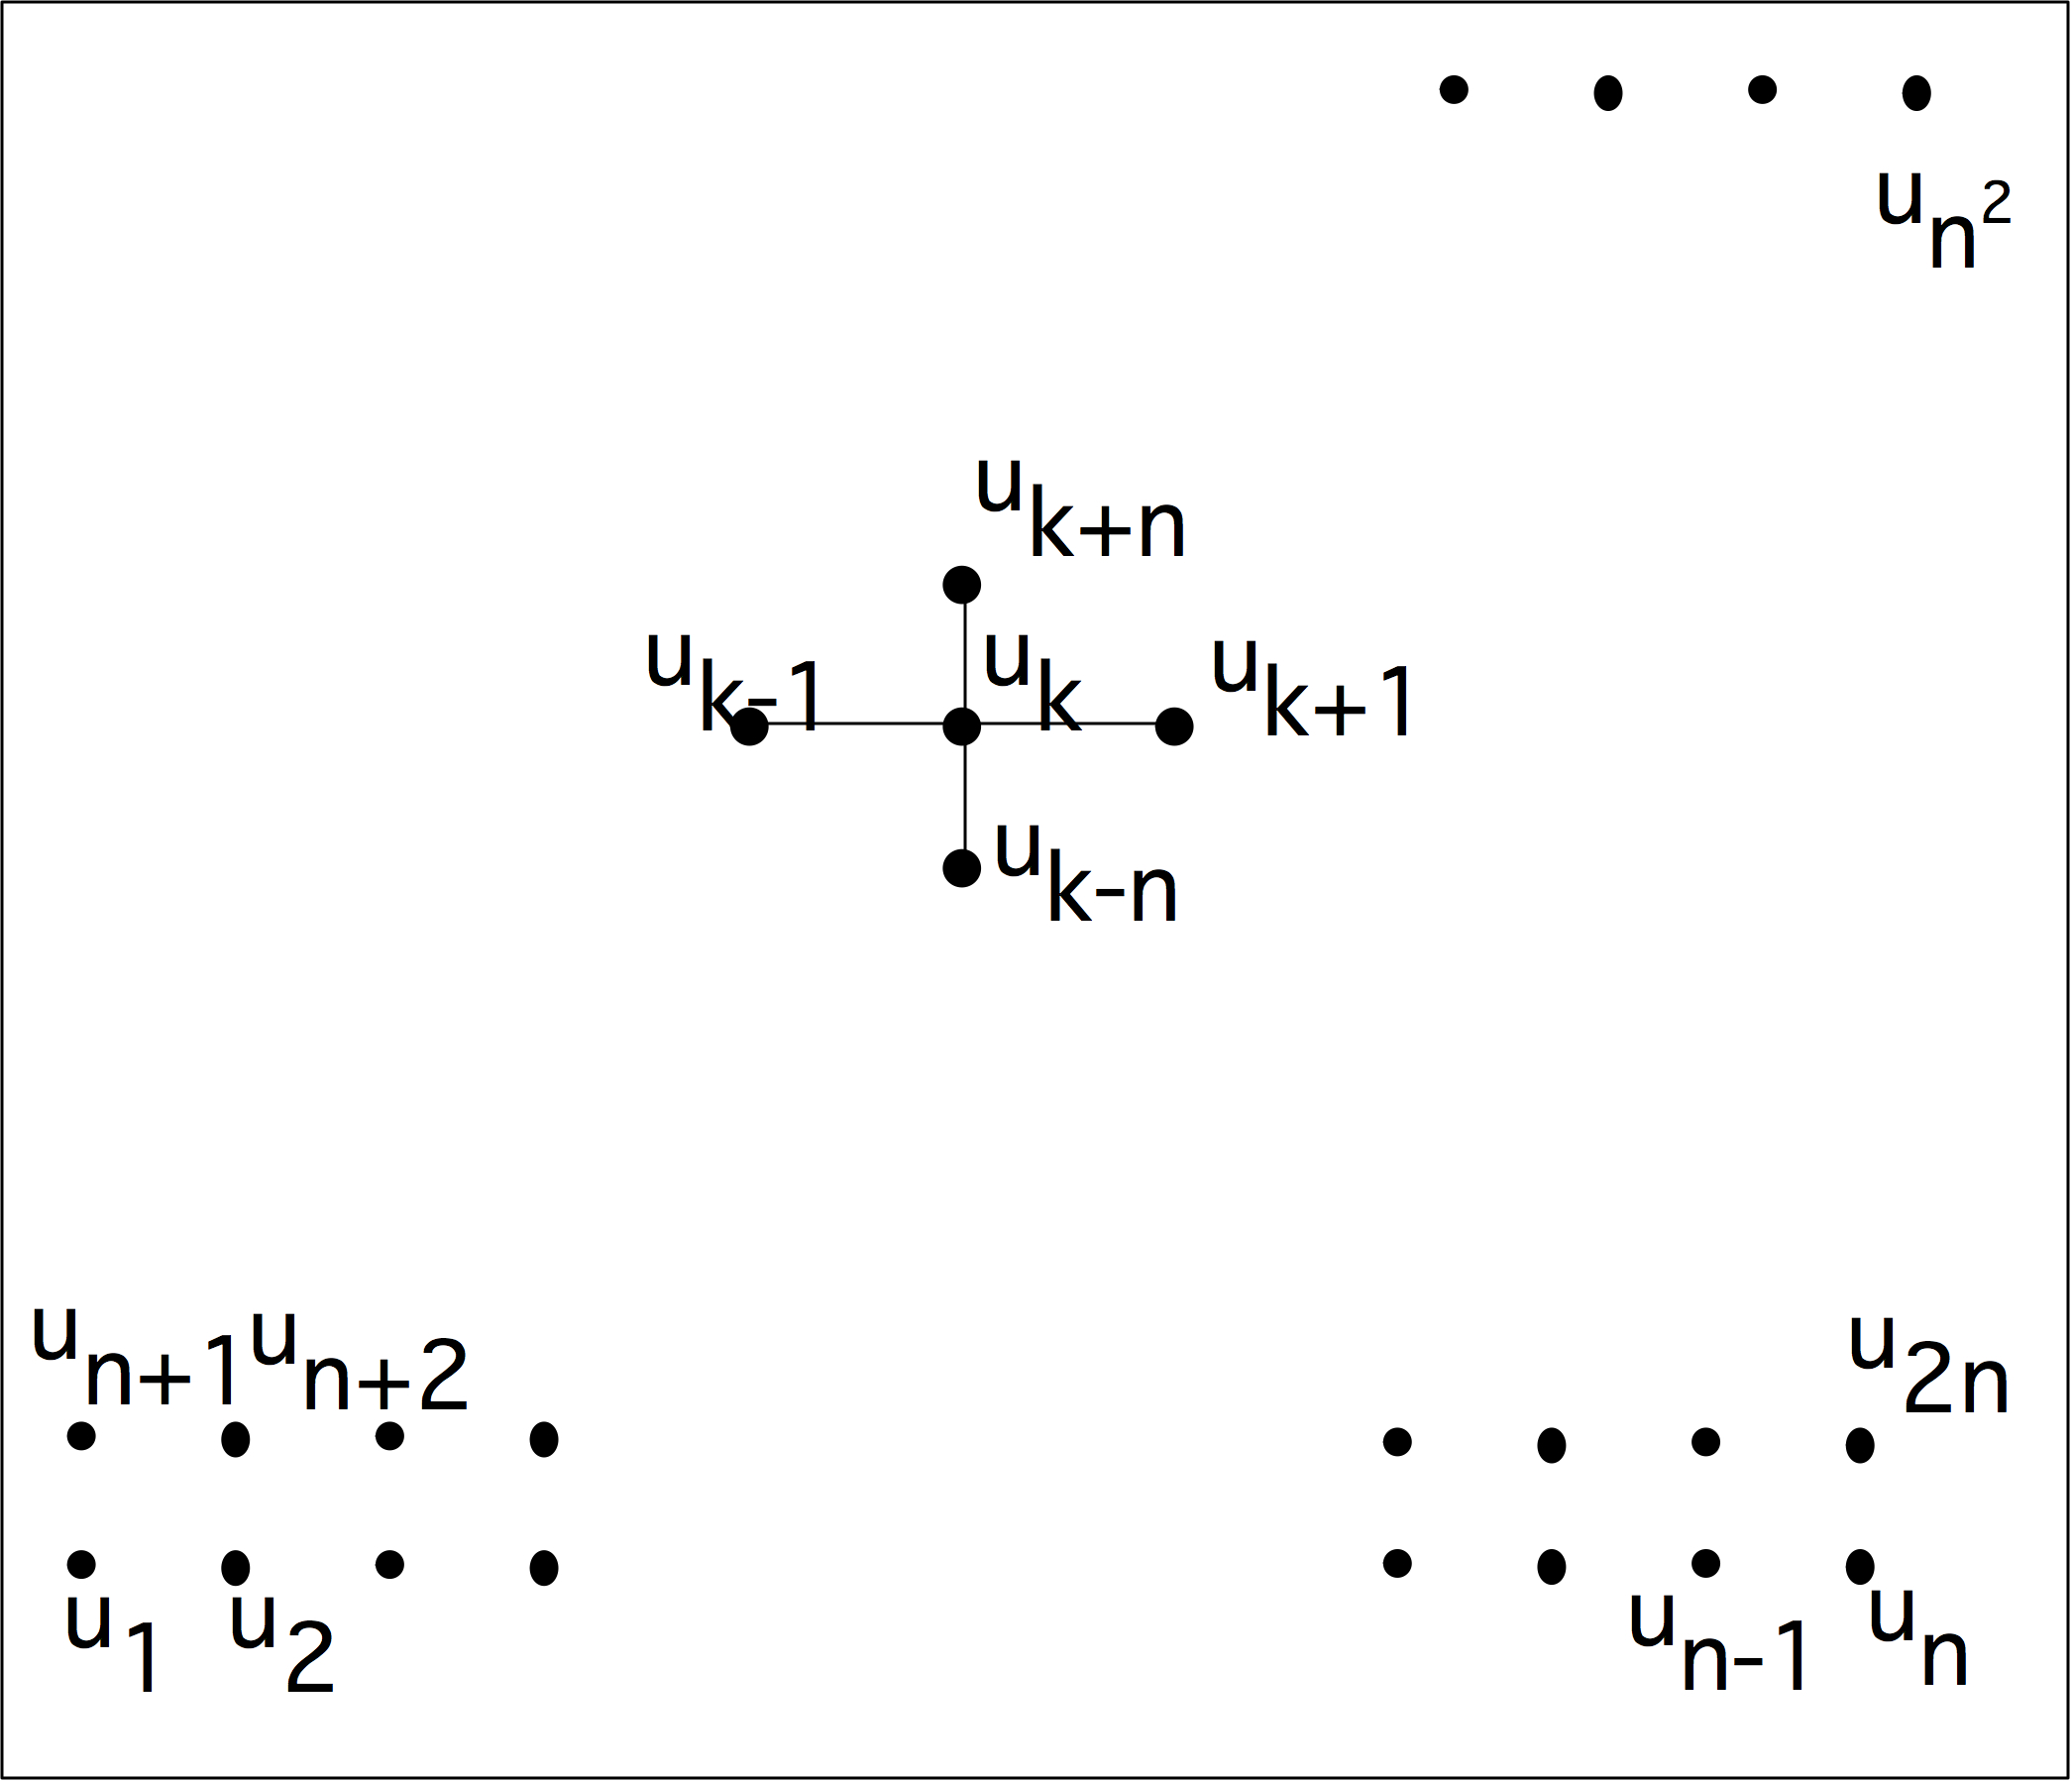
\includegraphics[scale=.11]{graphics-public/laplacedomain}
  \end{quote}
  \caption{A difference stencil applied to a two-dimensional square
    domain}
  \label{fig:laplacedomain}
\end{figure}
figure~\ref{fig:laplacedomain} pictures the variables in the domain,
and how 
equation~\eqref{eq:5-point-star-ij} relates them. From now on, when
making such a picture of the domain, we will
just use the indices of the variables, and omit the `$u$' identifier.

The matrix of equation~\ref{eq:5starmatrix} is banded as in the
one-dimensional case, but
unlike in the one-dimensional case, there are zeros inside the
band. (This has some important consequences when we try to solve the
linear system; see section~\ref{sec:fill}.) Because the matrix has five
nonzero diagonals, it is said to be of \indexterm{penta-diagonal}
structure.

You can also put a block structure on the matrix, by grouping the
unknowns together that are in one row of the domain. This is called a
\indexterm{block matrix}, and, on the block level, it
has a \indexterm{tridiagonal} structure, so we call this a
\indexterm{block tridiagonal} matrix. Note that the diagonal blocks
themselves are tridiagonal; the off-diagonal blocks are
minus the identity matrix.

%\Level 2 {Non-square domains}

This matrix, like the one-dimensional example above, has constant
diagonals, but this is again due to the simple nature of the
problem. In practical problems it will not be true. That said,
such `constant coefficient' problems occur, and when they are on
rectangular domains, there are very efficient methods for solving
the linear system with $N\log N$ time complexity.
\begin{figure}
  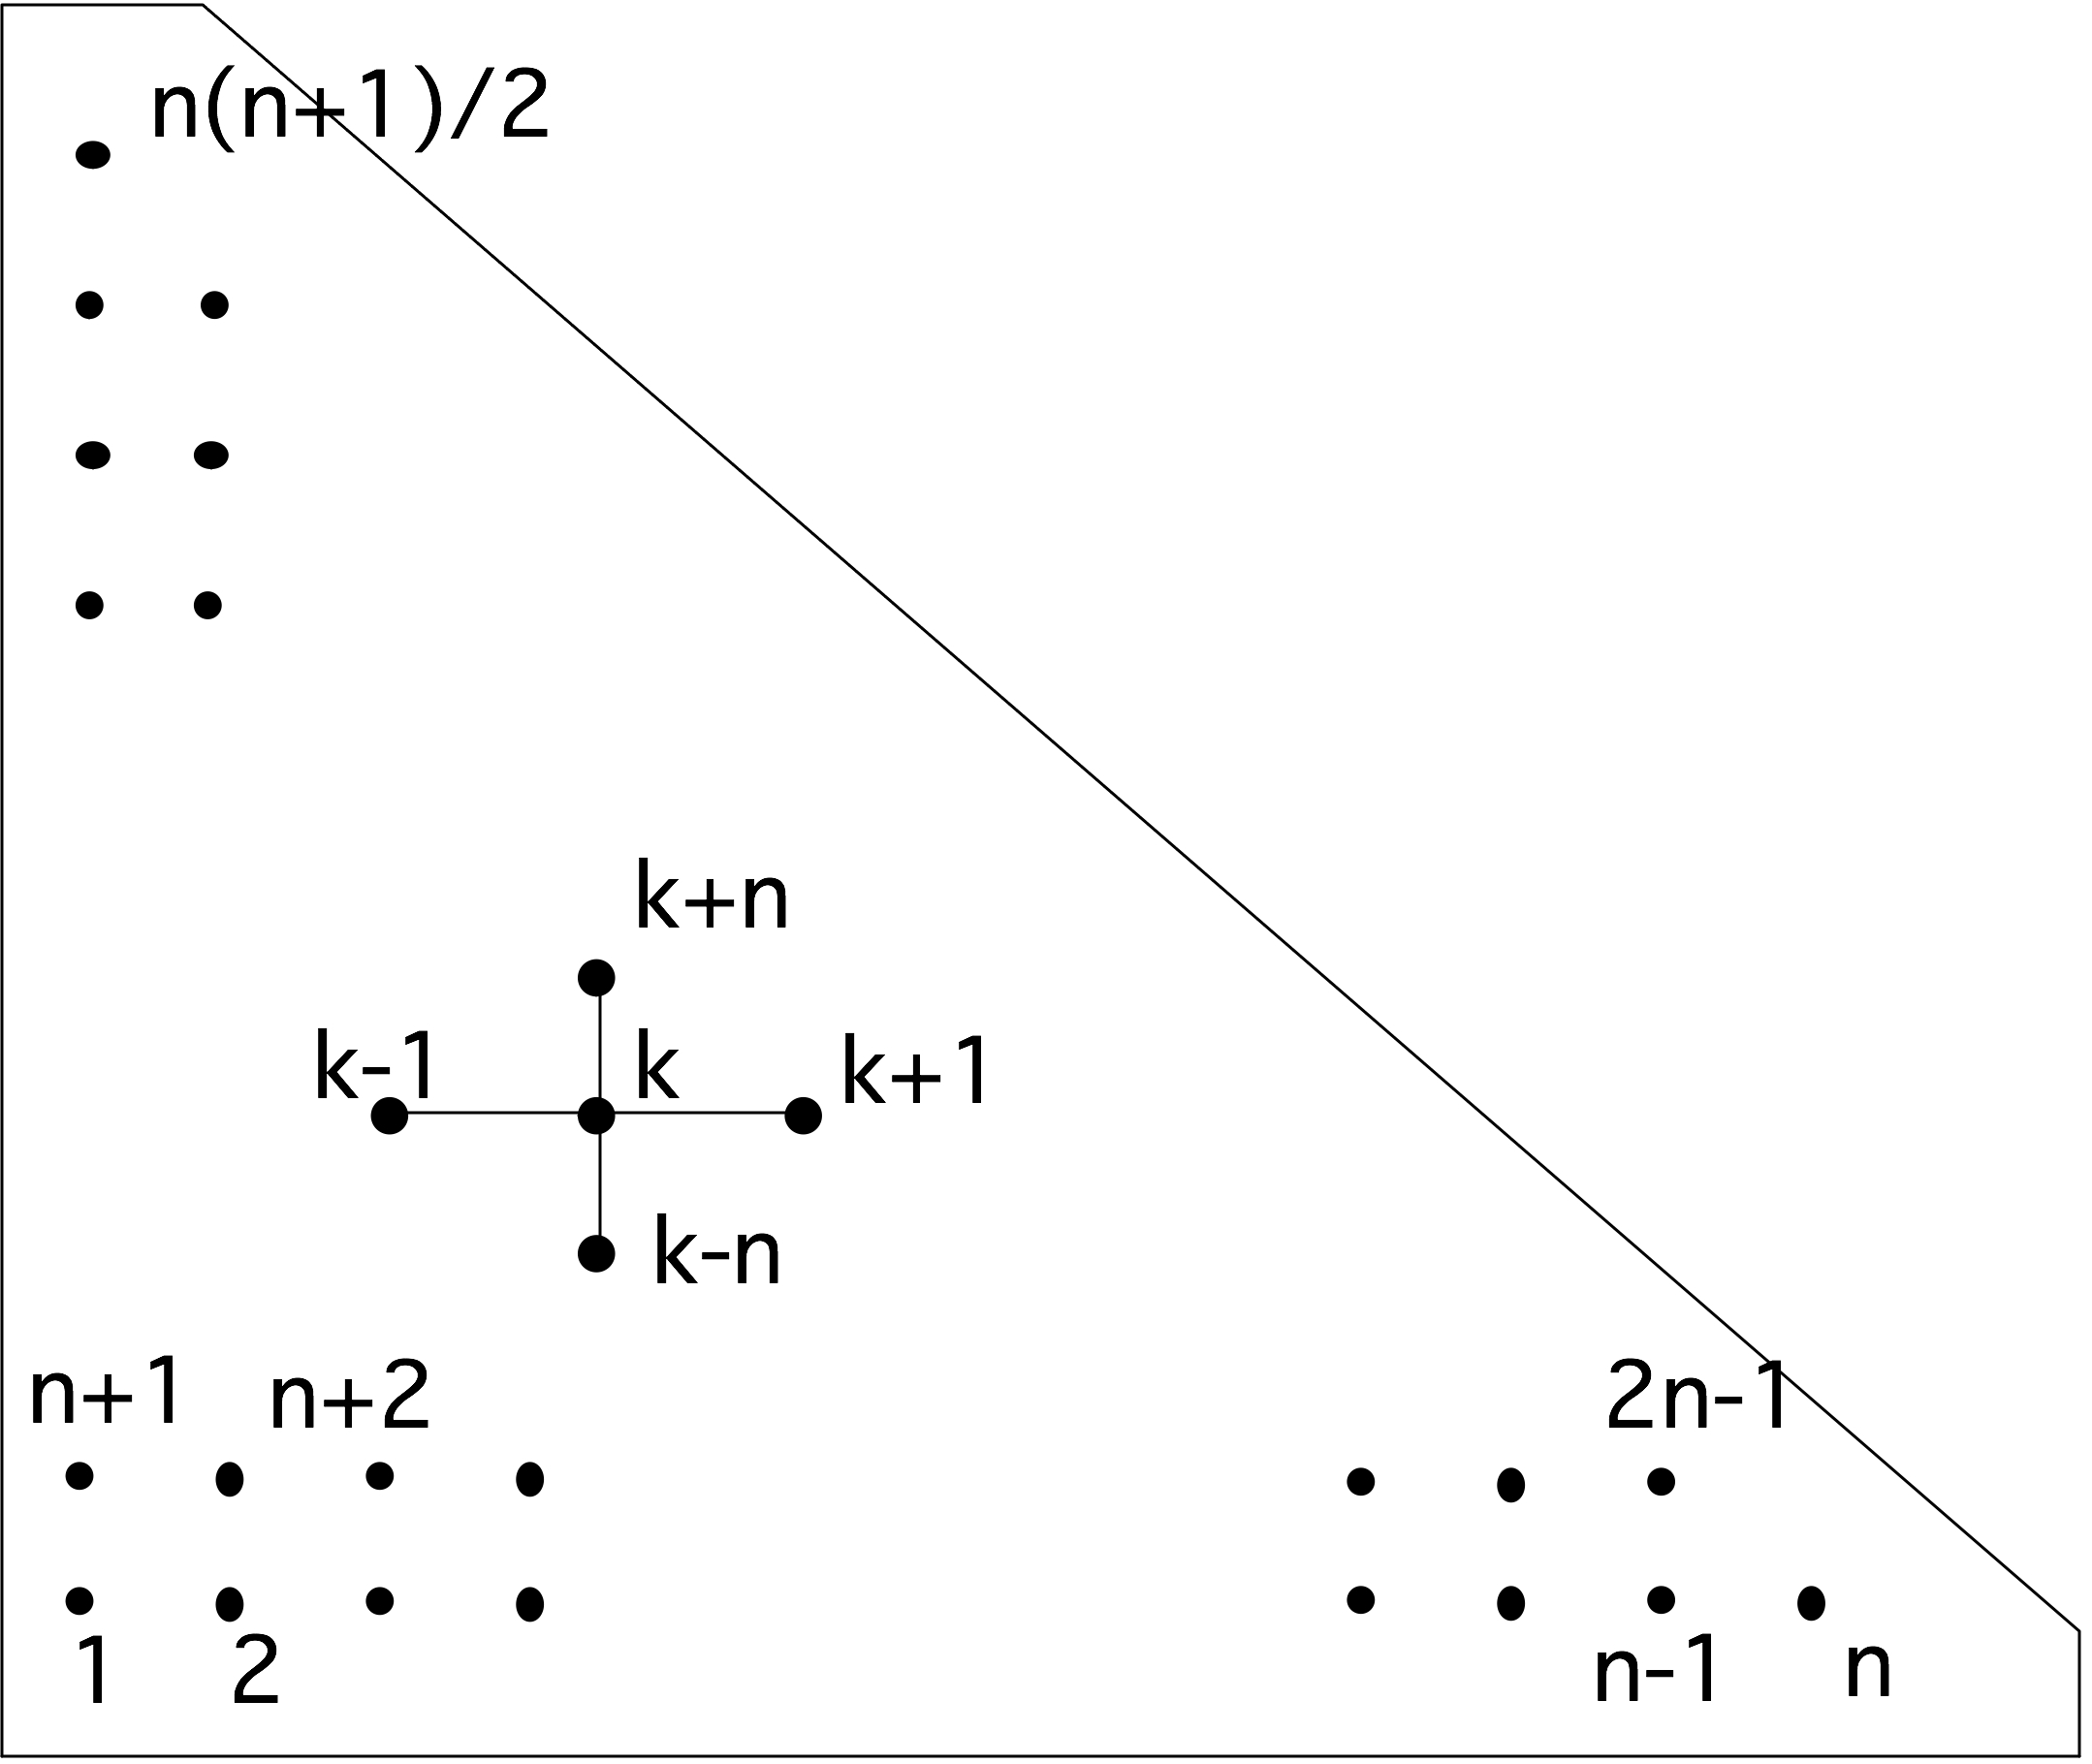
\includegraphics[scale=.1]{graphics-public/laplacetriangle}
  \caption{A triangular domain of definition for the Poisson equation}
  \label{fig:laplacetriangle}
\end{figure}

\begin{exercise}
  The block structure of the matrix, with all diagonal blocks having
  the same size, is due to the fact that we defined our \ac{BVP} on a
  square domain. Sketch the matrix structure that arises from
  discretizing equation~\eqref{eq:laplace}, again with central
  differences, but this time defined on a triangular domain; see
  figure~\ref{fig:laplacetriangle}. Show that, again, there is a block
  tridiagonal matrix structure, but that the blocks are now of varying
  sizes. Hint: start by sketching a small example. For $n=4$ you
  should get a $10\times 10$ matrix with a $4\times 4$ block structure.
\end{exercise}

For domains that are even more irregular, the matrix structure will
\begin{figure}[ht]
  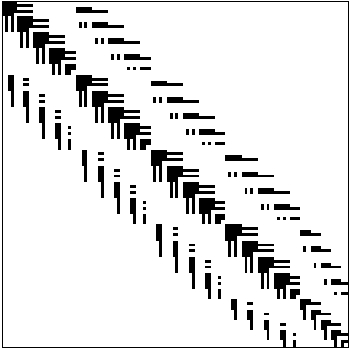
\includegraphics[scale=.6]{graphics-public/drivencavity}
  \caption{A matrix from an irregular problem}
  \label{fig:driven}
\end{figure}
also be irregular; see figure~\ref{fig:driven} for an example.

The regular block structure is also caused by our decision to order
the unknowns by rows and columns. This known as the \indexterm{natural
  ordering} or \indexterm{lexicographic ordering}; various other orderings are
possible. One common way of ordering the unknowns is the
\indexterm{red-black ordering} or \indexterm{checkerboard
  ordering} which has advantanges for parallel computation. This will
be discussed in section~\ref{sec:parallel-prec}.

There is more to say about analytical aspects of the \ac{BVP} (for
instance, how smooth is the solution and how does that depend on the
boundary conditions?) but those questions are outside the scope of
this course. Here we only focus on the numerical aspects of the
matrices. In the  chapter on linear algebra, we will come back to the
\ac{BVP}, since solving the linear system is mathematically interesting.

\Level 2 {Difference stencils}

The discretization \eqref{eq:5-point-star} is often phrased as
applying the \indexterm{difference stencil}
\[
\begin{matrix}
  \cdot&-1&\cdot\\ -1&4&-1\\ \cdot&-1&\cdot
\end{matrix}
\]
to the function~$u$. Given a physical domain, we apply the stencil to
each point in that domain to derive the equation for that
point. Figure~\ref{fig:laplacedomain} illustrates that for a square domain
of $n\times n$ points.
Connecting this figure with equation~\eqref{eq:5starmatrix}, you
see that the connections in the same line give rise to the main
diagonal and first upper and lower offdiagonal; the connections to the
next and previous lines become the nonzeros in the off-diagonal
blocks.

This particular stencil is often referred to as
the `5-point star'. There are other difference stencils; the structure
of some of them are depicted in figure~\ref{fig:stencils}.
\begin{figure}[ht]
  \centering
  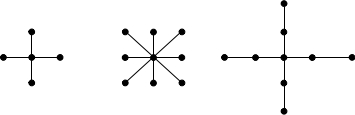
\includegraphics[scale=.8]{graphics-public/stencils}
  \caption{The structure of some difference stencils in two dimensions}
  \label{fig:stencils}
\end{figure}
A stencil with only connections in horizontal or vertical direction is
called a `star stencil', while one that has cross connections (such as
the second in figure~\ref{fig:stencils}) is called a `box
stencil'. 
\begin{exercise}
  Consider the third stencil in figure~\ref{fig:stencils}, used for a
  \ac{BVP} on a square domain.
  What does the sparsity structure of the resulting matrix look like,
  if we again order the variables by rows and columns?
\end{exercise}

Other stencils than the 5-point star can be used to attain higher
accuracy, for instance giving a truncation error of~$O(h^4)$. They can
also be used for other differential equations than the one discussed
above. For instance, it is not hard to show that for the equation
$u_{xxxx}+u_{yyyy}=f$ we need a stencil that contains both $x,y\pm h$
and $x,y\pm 2h$ connections, such as the third stencil in the
figure. Conversely, using the 5-point stencil no values of the
coefficients give a discretization of the fourth order problem with
less than~$O(1)$ truncation error.

While the discussion so far has been about two-dimensional
problems, it is easily generalized to higher dimensions for such
equations as $-u_{xx}-u_{yy}-u_{zz}=f$. The straightforward
generalization of the 5-point stencil, for instance, becomes a 7-point
stencil in three dimensions.

\Level 2 {Other discretization techniques}
\label{sec:fem}

In the above, we used the \ac{FDM} to find a numerical solution
to a differential equation. There are various other techniques, and in
fact, in the case of boundary value problems, they are usually
preferred over finite differences. The most popular methods are the
\indexac{FEM} and the \indexterm{finite volume
  method}. Especially the finite element method is attractive, since
it can handle irregular shapes more easily, and it is more amenable to
approximation error analysis. However, on the simple problems discussed here
it gives similar or even the same linear systems as \ac{FD} methods,
so we limit the discussion to Finite Differences, since we are mostly
concerned with the computational aspects of the linear systems.

There will be a brief discussion of finite element matrices in
section~\ref{sec:fem-assembly}.

\indexacend{BVP}

\Level 0 {Initial boundary value problem}
\label{sec:heateq}
\indexacstart{IBVP}

We will now go on to discuss an \acf{IBVP}, which, as you may deduce
from the name, combines aspects of \ac{IVP}s and \ac{BVP}s. Here we
will limit ourselves to one space dimension.

The problem we are considering is that of  heat conduction in a rod, where
$T(x,t)$ describes the temperature in location~$x$ at time~$t$, for
$x\in[a,b]$, $t>0$. The so-called \indexterm{heat equation} (see
Appendix~\ref{app:pde} for a quick introduction to \acp{PDE} in
general and the heat equation in particular) is:
\[
  \frac\partial{\partial t}T(x,t)-\alpha\frac{\partial^2}{\partial x^2}T(x,t)
  =q(x,t) 
\]
where
\begin{itemize}
\item The initial condition $T(x,0)=T_0(x)$ describes the initial
  temperature distribution.
\item The boundary conditions $T(a,t)=T_a(t)$, $T(b,t)=T_b(t)$
  describe the ends of the rod, which can for instance be fixed to an
  object of a known temperature.
\item The material the rod is made of is modeled by a single parameter
  $\alpha>0$, the thermal diffusivity, which describes how fast heat
  diffuses through the material.
\item The forcing function $q(x,t)$ describes externally applied
  heating, as a function of both time and place.
\end{itemize}
There is a simple connection between the \ac{IBVP} and the \ac{BVP}:
if the boundary functions $T_a$ and $T_b$ are constant, and $q$~does
not depend on time, only on location, then intuitively $T$~will
converge to a \indexterm{steady state}. 
The equation for this is $-\alpha u''(x)=q$.

\def\fr{\frac{\alpha\Delta t}{\Delta x^2}}

\Level 1 {Discretization}

We now discretize both space and time, by $x_{j+1}=x_j+\Delta x$ and
$t_{k+1}=t_k+\Delta t$, with boundary conditions $x_0=a$, $x_n=b$, 
and $t_0=0$. We write $T^k_j$ for the numerical solution at $x=x_j,t=t_k$;
with a little luck, this will approximate the exact
solution $T(x_j,t_k)$.

For the space discretization we use the central difference formula
\eqref{eq:2nddiff-formula}:
\[ 
  \left.\frac{\partial^2}{\partial x^2}T(x,t_k)\right|_{x=x_j} 
  \Rightarrow
  \frac{T_{j-1}^k-2T_j^k+T_{j+1}^k}{\Delta x^2}.
\]
For the time discretization we can use any of the schemes in
section~\ref{sec:fd-ode}. We will investigate again the explicit and
implicit schemes, with similar conclusions about the
resulting stability.

\Level 2 {Explicit scheme}

With explicit time stepping we approximate the time derivative as
\begin{equation}
  \left.\frac\partial{\partial t}T(x_j,t)\right|_{t=t_k}
  \Rightarrow
  \frac{T_j^{k+1}-T_j^k}{\Delta t}.
  \label{eq:disc-time-explicit}
\end{equation}
Taking this together with the central differences in space, we now have
\[
  \frac{T_j^{k+1}-T_j^k}{\Delta t}-\alpha
  \frac{T_{j-1}^k-2T_j^k+T_{j+1}^k}{\Delta x^2}=q_j^k 
\]
which we rewrite as
\begin{equation}
  \label{eq:bivp-explicit}
  T_j^{k+1}=T_j^k+\fr
  (T_{j-1}^k-2T_j^k+T_{j+1}^k)+\Delta t q_j^k 
\end{equation}
Pictorially, we render this as a difference stencil in
figure~\ref{fig:Euler-forward-stencil}.
\begin{figure}
  \leavevmode\kern\unitindent 
  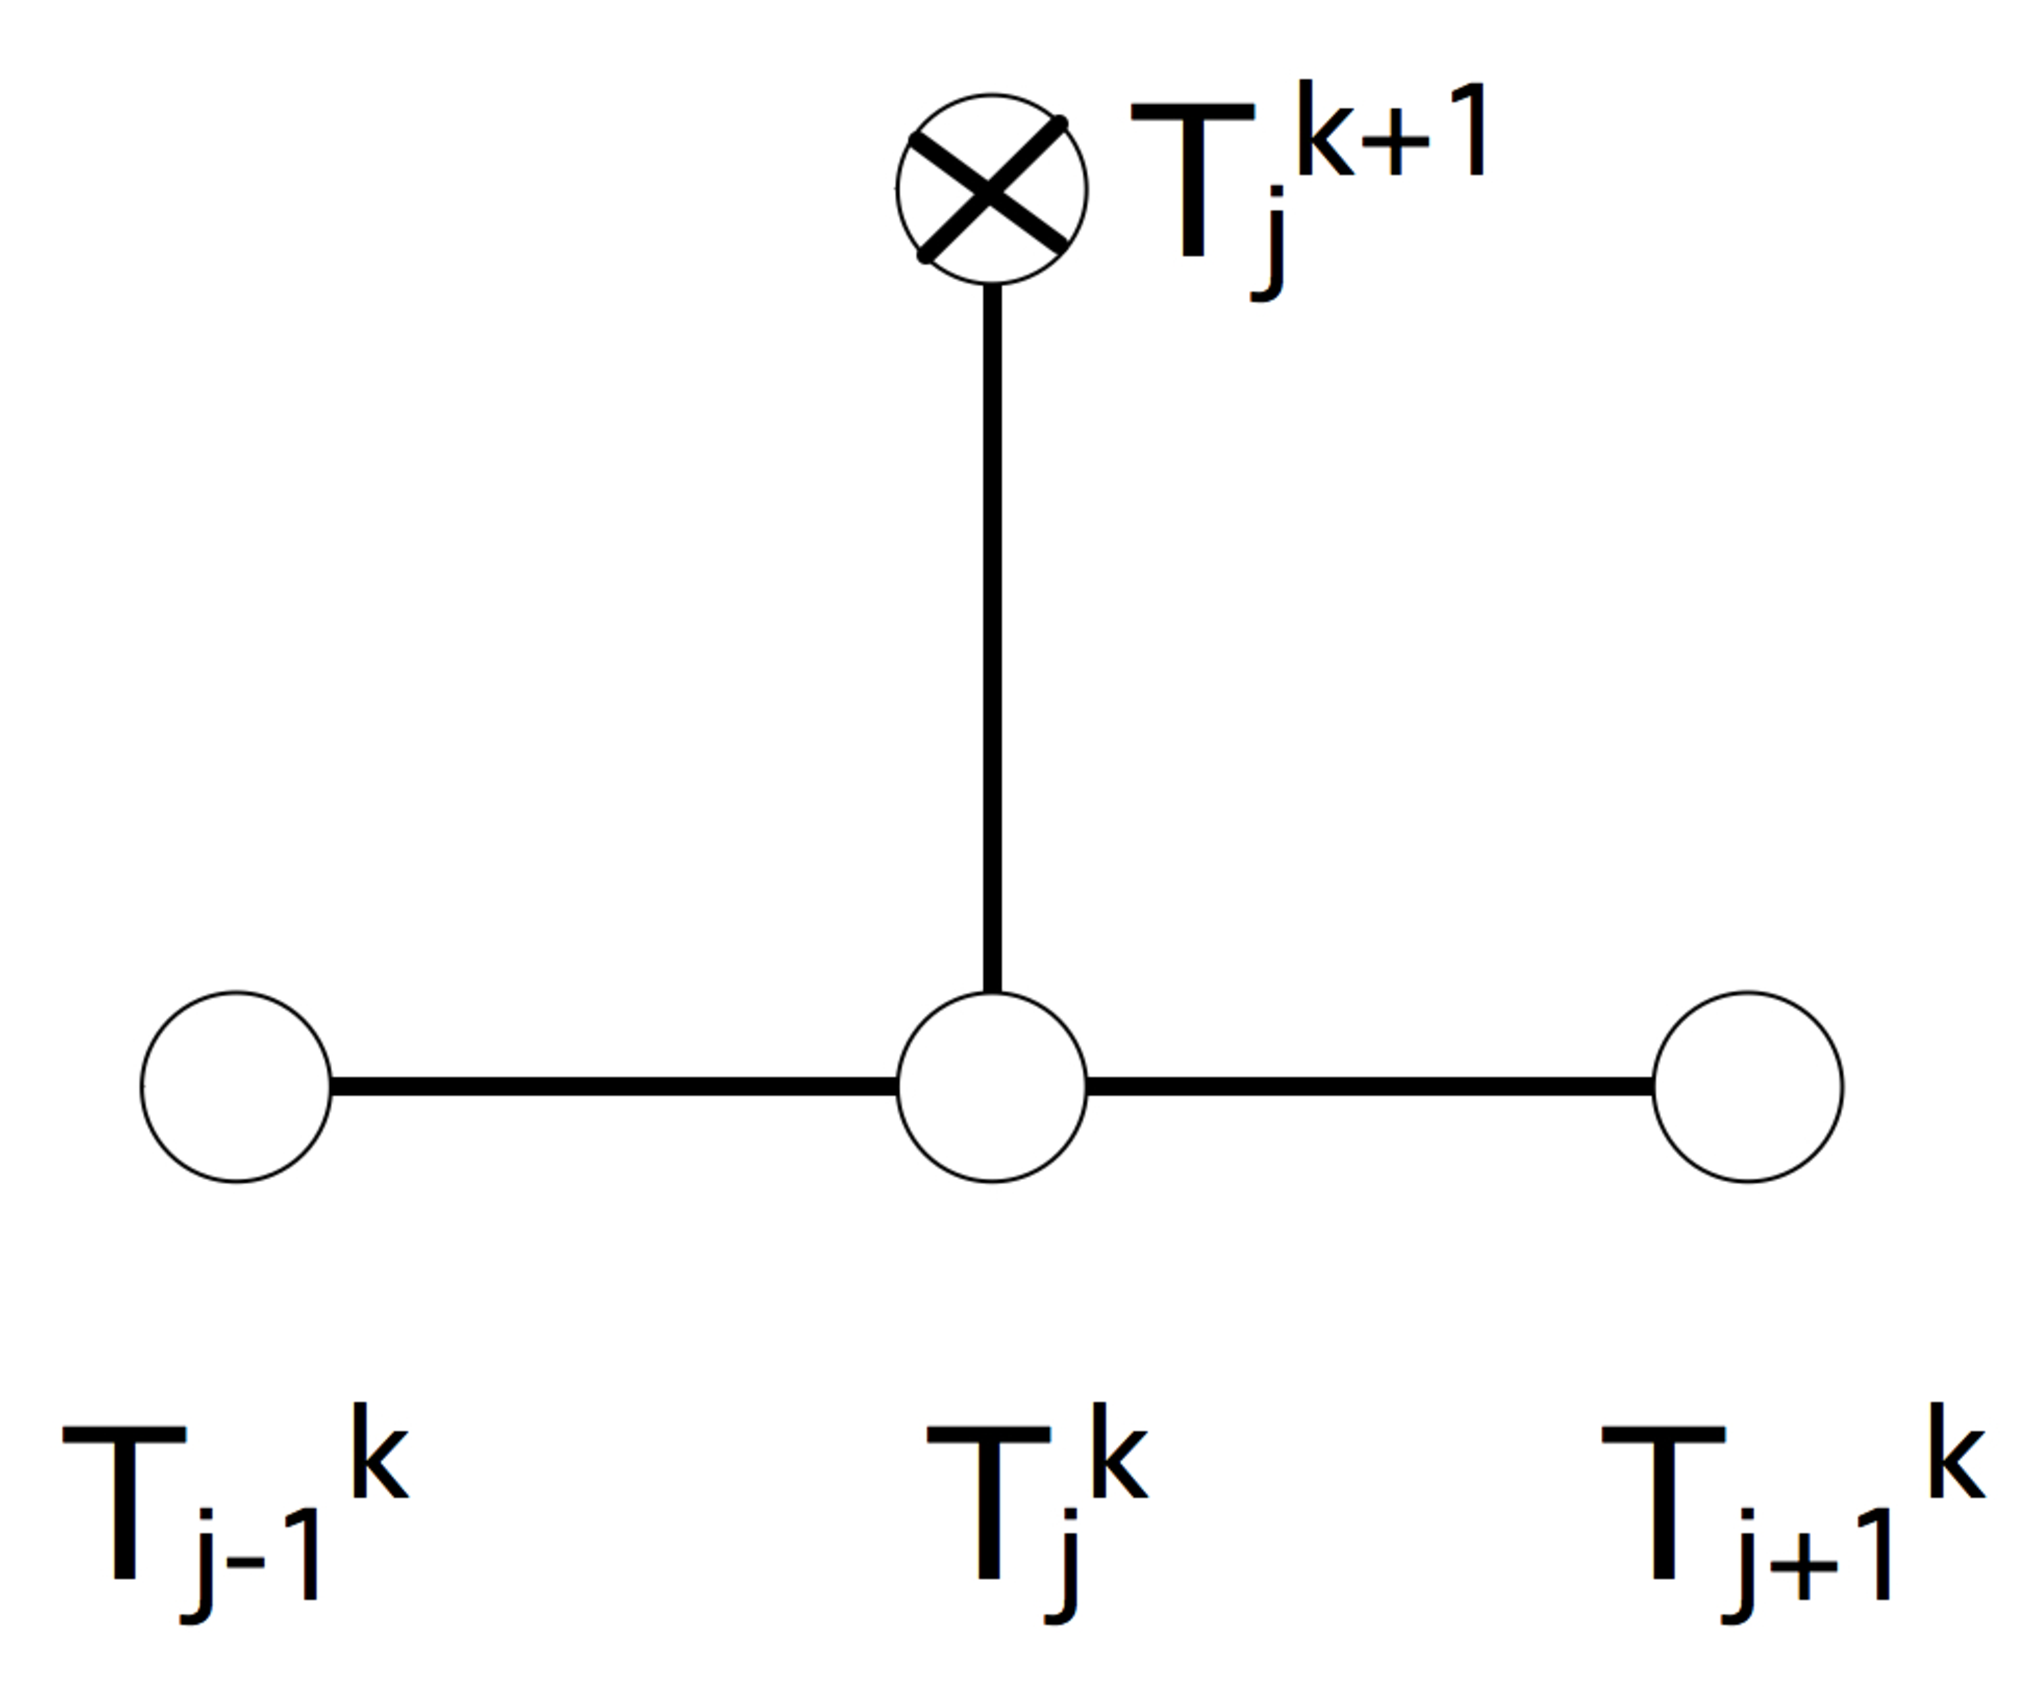
\includegraphics[scale=.15]{graphics-public/euler-forwardpdf}
  \caption{The difference stencil of the Euler forward method for the
    heat equation}
  \label{fig:Euler-forward-stencil}.
\end{figure}
This expresses that the function value in each point is determined by
a combination of points on the previous time level.

It is convenient to summarize the set of equations
\eqref{eq:bivp-explicit} for a given~$k$ and all values of~$j$
in vector form as
\begin{equation}
  \label{eq:bivp-explicit-vector}  
   T^{k+1}=\left(I-\fr K\right)
   T^k+\Delta t q^k 
\end{equation}
where
\[
  K=
  \begin{pmatrix}
    2&-1\\ -1&2&-1\\ &\ddots&\ddots&\ddots
  \end{pmatrix},\qquad
  T^k=
  \begin{matrix}
    T^k_1\\ \vdots \\ T^k_n
  \end{matrix}.
\]
The important observation here is that the dominant computation for
deriving the vector $T^{k+1}$ 
from $ T^k$ is a simple matrix-vector multiplication:
\[ T^{k+1}\leftarrow AT^k+\Delta tq^k \]
where $A=I-\fr K$. This is a first indication that the sparse
matrix-vector product is an important operation; see sections
\ref{sec:sparse} and~\ref{sec:pspmvp}.
Actual
computer programs using an explicit method often do not form the
matrix, but evaluate the equation~\eqref{eq:bivp-explicit}. However,
the linear algebra formulation~\eqref{eq:bivp-explicit-vector}
is more insightful for purposes of analysis.

\Level 2 {Implicit scheme}

In equation \eqref{eq:disc-time-explicit} we let $T^{k+1}$ be defined
from~$T^k$. We can turn this around by defining $T^k$ from~$T^{k-1}$,
as we did for the \ac{IVP} in section~\ref{sec:implicit-euler}. For
the time discretization this gives
\begin{equation}
  \left.\frac\partial{\partial t}T(x,t)\right|_{t=t_k}
  \Rightarrow
  \frac{T_j^k-T_j^{k-1}}{\Delta t}
  \qquad\hbox{or}\qquad
  \left.\frac\partial{\partial t}T(x,t)\right|_{t=t_{k+1}}
  \Rightarrow
  \frac{T_j^{k+1}-T_j^k}{\Delta t}.
  \label{eq:heat-time-explicit}
\end{equation}
The implicit time step discretization of the whole heat equation,
evaluated in~$t_{k+1}$, now becomes:
\[
  \frac{T_j^{k+1}-T_j^k}{\Delta t}-\alpha
  \frac{T_{j-1}^{k+1}-2T_j^{k+1}+T_{j+1}^{k+1}}{\Delta x^2}=q_j^{k+1} 
\]
or
\begin{equation}
  \label{eq:bivp-implicit}
  T_j^{k+1}-\fr
  (T_{j-1}^{k+1}-2T_j^{k+1}+T_{j+1}^{k+1})=T_j^k+\Delta t q_j^{k+1}
\end{equation}
Figure~\ref{fig:Euler-backward-stencil} renders this as a stencil;
this expresses that each point on the current time level influences a
combination of points on the next level.
\begin{figure}
  \leavevmode\kern\unitindent 
  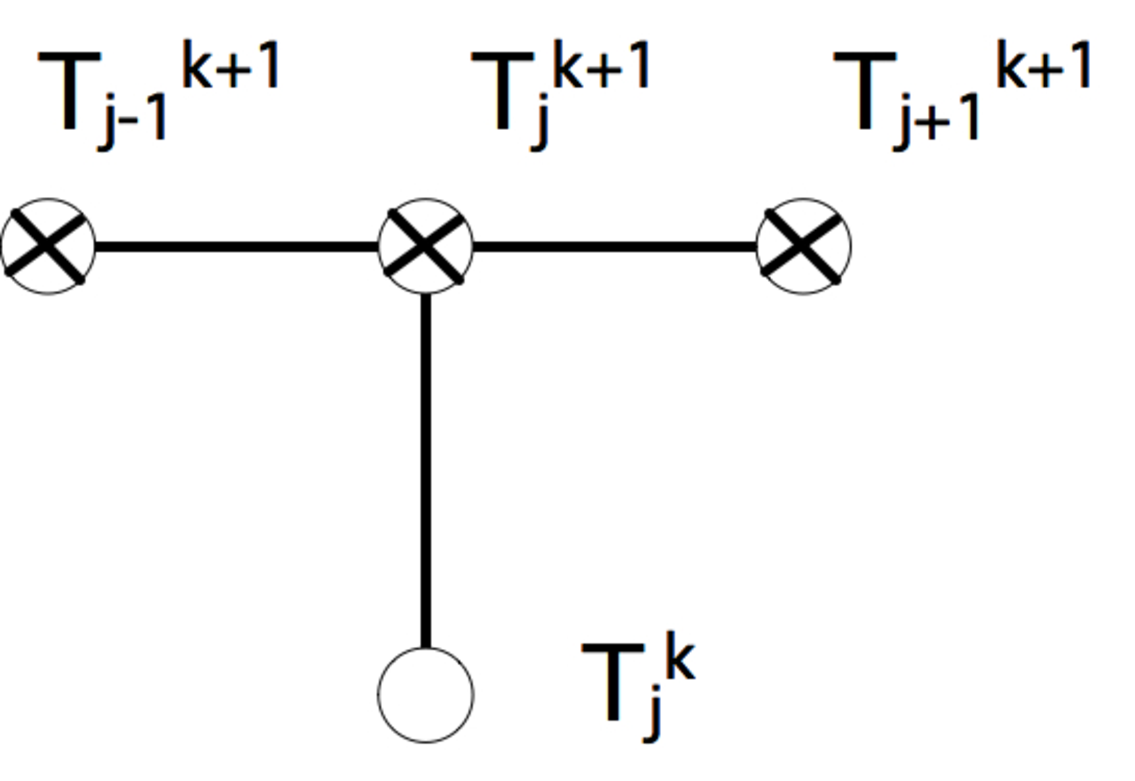
\includegraphics[scale=.25]{graphics-public/euler-backwardpdf}
  \caption{The difference stencil of the Euler backward method for the
    heat equation}
  \label{fig:Euler-backward-stencil}.
\end{figure}
Again we write this in vector form:
\begin{equation}
  \label{eq:bivp-implicit-vector}
  \left(I+\fr K\right) T^{k+1}=
   T^k+\Delta t q^{k+1}
\end{equation}
As opposed to the explicit method, where a matrix-vector
multiplication sufficed, the derivation of the vector $ T^{k+1}$ 
from $ T^k$ now involves solving a linear system
\[ T^{k+1}\leftarrow A\inv (T^k+\Delta tq^{k+1}) \]
where $A=I+\fr K$, a harder operation than the matrix-vector
multiplication.  In this case, it is not possible, as above, to
evaluate the equation~\eqref{eq:bivp-implicit} directly. Codes using an
implicit method actually form the coefficient matrix, and solve the
system~\eqref{eq:bivp-implicit-vector} as such. Solving linear systems
will be the focus of much of chapters \ref{ch:linear}
and~\ref{ch:parallellinear}.

\begin{exercise}
  Show that the flop count for a time step of the implicit method is
  of the same order as of a time step of the explicit method. (This
  only holds for a problem with one space dimension.) Give at least
  one argument why we consider the implicit method as computationally
  `harder'.
\end{exercise}

The numerical scheme that we used here is of first order in time and
second order in space: the truncation error (section~\ref{sec:fd-ode})
is $O(\Delta t+\Delta x^2)$. It would be possible to use a scheme that
is second order in time by using central differences in time
too. Alternatively, see exercise~\ref{ex:crank}.

\Level 1 {Stability analysis}

We now analyse the stability of the explicit and implicit
schemes in a simple case. Let $q\equiv0$, and assume
$T_j^k=\beta^ke^{i\ell x_j}$ for some~$\ell$\footnote{Actually,
  $\beta$ is also dependent on~$\ell$, but we will save ourselves a
  bunch of subscripts, since different $\beta$ values never appear
  together in one formula.}. This assumption is intuitively
defensible: since the differential equation does not `mix' the $x$ and
$t$ coordinates, we surmise that the solution will be a product
$T(x,t)=v(x)\cdot w(t)$ of the
separate solutions of
\[
\begin{cases}
  v_{xx}=c_1 v,&v(0)=0,\,v(1)=0\\
  w_t=c_2 w & w(0)=1\\
\end{cases}
\]
The only meaningful solution occurs with $c_1,c_2<0$, in which case we
find:
\[ v_{xx}=-c^2v \Rightarrow v(x)=e^{-icx}=e^{-i\ell\pi x} \]
where we substitute $c=\ell\pi$ to take boundary conditions into
account,
and 
\[ w(t) = e^{-ct} = e^{-ck\Delta t} = \beta^k,\quad \beta=e^{-ck}. \]
If the assumption on this form of the solution holds up, we need
$|\beta|<1$ for stability.

Substituting the surmised form for $T_j^k$ into the  explicit scheme gives
  \begin{eqnarray*}
    T_j^{k+1}&=&T_j^k+\fr(T_{j-1}^k-2T_j^k+T_{j+1}^k)\\
    \Rightarrow \beta^{k+1}e^{i\ell x_j}&=&\beta^ke^{i\ell x_j}
    +\fr (\beta^ke^{i\ell x_{j-1}}-2\beta^ke^{i\ell x_j}+\beta^ke^{i\ell x_{j+1}})\\
    &=&\beta^ke^{i\ell x_j}\left[1+\fr\left[e^{-i\ell\Delta x}-2+e^{i\ell\Delta x}\right]\right]\\
    \Rightarrow \beta&=&
    1+2\fr[\frac12(e^{i\ell\Delta x}+e^{-\ell\Delta x})-1]\\
    &=&1+2\fr(\cos(\ell\Delta x)-1)
  \end{eqnarray*}

For stability we need $|\beta|<1$:
  \begin{itemize}
  \item $\beta<1\Leftrightarrow 2\fr(\cos(\ell\Delta x)-1)<0$: this is
    true for any $\ell$ and any choice of $\Delta x,\Delta t$.
  \item $\beta>-1\Leftrightarrow 2\fr(\cos(\ell\Delta x)-1)>-2$: this
    is true for all~$\ell$ only if $2\fr<1$, that is
    \[ \Delta t<\frac{\Delta x^2}{2\alpha} \]
  \end{itemize}
The latter condition poses a big restriction on the allowable size of
the time steps: time steps have to be small enough for the method to
be stable. This is similar to the stability analysis of the explicit
method for the \ac{IVP}; however, now the time step is also related to
the space discretization. This implies that, if we decide we need more
accuracy in space and we halve the space discretization~$\Delta x$,
the number of time steps will be multiplied by four.

Let us now consider the stability of the implicit scheme.
Substituting the form of the solution $T_j^k=\beta^ke^{i\ell x_j}$
into the numerical scheme gives
  \begin{eqnarray*}
    T_j^{k+1}-T_j^k&=&\fr(T_{j_1}^{k+1}-2T_j^{k+1}+T_{j+1}^{k+1})\\
    \Rightarrow \beta^{k+1}e^{i\ell \Delta x}-\beta^ke^{i\ell x_j}&=&
    \fr(\beta^{k+1}e^{i\ell x_{j-1}}-2\beta^{k+1}e^{i\ell x_j}
    +\beta^{k+1}e^{i\ell x_{j+1}})
  \end{eqnarray*}
Dividing out $e^{i\ell x_j}\beta^{k+1}$ gives
  \begin{eqnarray*}
    &&1=\beta\inv+2\alpha\frac{\Delta t}{\Delta x^2}(\cos\ell\Delta
    x-1)\\
    &&\beta=\frac1{1+2\alpha\frac{\Delta t}{\Delta x^2}(1-\cos\ell\Delta x)}
  \end{eqnarray*}
Since $1-\cos\ell\Delta x\in(0,2)$, the denominator is strictly~$>1$.
Therefore the condition $|\beta|<1$ is always satisfied, regardless
the value of $\ell$ and the choices
of $\Delta x$ and~$\Delta t$: the method is always stable.

\begin{exercise}
  \label{ex:crank}
  The schemes we considered here are of first order in time and second
  order in space: their discretization order are $O(\Delta t)+O(\Delta
  x^2)$. Derive the \indexterm{Crank-Nicolson method} that is obtained
  by averaging the explicit and implicit schemes, show that it is
  unconditionally stable, and of second order in time.
\end{exercise}

\indexacend{PDE}
\indexacend{IBVP}
